\chapter{Sonstige Distributed-Ledger-Technologie}
\section{Directed Acyclic Graph}
Bei einem DAG handelt es sich um eine gerichteten azyklischen Graphen, der im Bereich der  Distributed-Ledger-Technologie dazu eingesetzt wird Transaktionen zu speichern.
Die Kryptowährung IOTA\footnote{\url{https://www.iota.org/}} setzt solch eine Datenstruktur ein. Der Konsens entsteht nicht durch eine Blockchain auf die sich alle Teilnehmer mithilfe der Konsnensregeln einigen. Der Konsens entsteht dadurch, dass Teilnehmer neue Transaktionen nur auf Transaktionen aufbauen, die sie für gültig halten. Um eine Transaktion in den Graphen zu schreiben, muss der Absender Proof-of-Work erledigen. 

\begin{figure}[H]
\centering
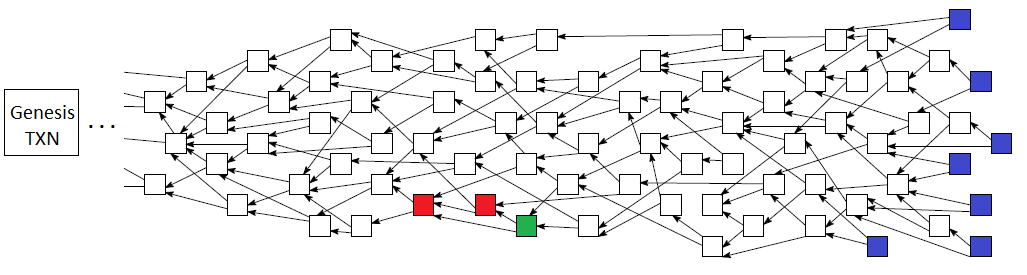
\includegraphics[width=1\linewidth]{Figures/tangle}
\decoRule
\caption{Directed Acyclic Graph}
\label{fig:tangle}
\end{figure}

Die grüne Transaktion aus Abbildung \ref{fig:tangle} baut auf den beiden roten Transaktionen auf und bestätigt diese auf diese Art und Weise. Je tiefer eine Transaktion im Graphen steckt, desto mehr Proof-of-Work baut auf ihr auf. Am rechten Rand befinden sich in blau neue, unbestätigte Transaktionen.
Kryptowährungen auf Basis solch einer Datenstruktur sind nicht für die Gewinnerauswahl einer Glücksspielanwendung nutzbar, da man sich nicht bereits im Vorfeld auf ein eindeutiges, in der Zukunft liegendes, aber dennoch zufälliges Ereignis einigen kann. Weiterführende Informationen zu IOTA und einer genaue Beschreibung der DAG Datenstruktur findet man unter \citep{tangle_whitepaper}.
\section{Konsensalgorithmus: Proof of stake }\label{pos}
Hier kann man auch noch erwähnen, dass Proof of stake und solche slotbasierten Ansätze nicht geeignet sind da der Slotleader direkten Einfluss nehmen kann.
\section{Payment Channels und Lightning Network}
Hier könnte man darauf eingehen, dass off-chain Transaktionen nicht einsetzbar sind, da die restlichen Teilnehmer somit nicht die Einzahlung überprüfen können.